\documentclass[11pt,a4paper]{article}
\usepackage[T1]{fontenc}
\usepackage[margin=2.3cm]{geometry}
\usepackage{amsmath,amssymb}
\usepackage{graphicx}
\usepackage[dvipsnames]{xcolor}
\usepackage{enumitem}
\usepackage[colorlinks=true,linkcolor=blue,urlcolor=blue]{hyperref}
\setlength{\parskip}{0.6em}
\setlength{\parindent}{0pt}
\begin{document}

\begin{center}{\LARGE\bfseries openprojectile}\\[0.4em]{\large Plan a cricket shot with air drag, in three sessions.}\\[0.2em]\small PAN IIT OSS explainer \textbullet{} secondary school to diploma / undergraduate (levels 3-5)\end{center}

\section*{Why this exists}
A ball in flight is the simplest moving system with two forces at work: gravity, which gives the neat parabola, and air drag, which spoils it and forces us to simulate. This explainer follows the ball from independent motions, through the range formula, to a validated numerical solution.

\section*{The end goal}
Plan a cricket shot with air drag. The end goal is planning a cricket shot with air drag: given a boundary distance, a wind and a ball, choose the launch speed and angle. The same method plans a golf drive, a football kick or a water jet.

\section*{How the three sessions build up}
\begin{enumerate}[nosep]
\item \textbf{Session 1: Throw a ball: two independent motions} (Level 1, conceptual interactive model, 60 min).
\item \textbf{Session 2: The equations: range, best angle and a design problem} (Level 2, mathematical engineering model, 75 min).
\item \textbf{Session 3: Air drag: an RK4 simulation, validated} (Level 3, simulation and validation, 90 min).
\end{enumerate}

\section{Session 1: Throw a ball: two independent motions}

\subsection*{A. Real-world problem}
A fielder throws the ball to the wicket keeper; a batter lofts it towards the boundary. How far does it go, how high does it get and how long does it hang in the air? The surprise that makes this easy: the sideways motion and the up-and-down motion do not disturb each other, so we can handle them one at a time and then put them together.

\subsection*{B. Concept and theory}
A ball leaves the hand with speed v at an angle a above the horizontal. Its velocity splits into a sideways part vx = v cos(a) and an upward part vy = v sin(a). Sideways nothing pushes the ball (we ignore air), so vx never changes and x = vx t. Up and down gravity pulls with acceleration g, so vy falls steadily and y = vy t - g t\textasciicircum{}2 / 2. The ball stops rising when vy - g t = 0, which happens at t = vy / g. It takes as long to come down, so the time in the air is T = 2 vy / g, the peak height is H = vy\textasciicircum{}2 / (2 g) and the range is R = vx T.

\begin{itemize}[nosep]
\item v: launch speed (m/s)
\item a: launch angle above the horizontal (degrees)
\item vx, vy: horizontal and vertical parts of the launch velocity (m/s)
\item g: acceleration of gravity (9.81) (m/s\textasciicircum{}2)
\item T, H, R: time of flight, peak height, range (s, m, m)
\item t: time since launch (s)
\end{itemize}

\begin{equation*}
v_x=v\cos a,\qquad v_y=v\sin a
\end{equation*}

\begin{equation*}
x=v_x\,t,\qquad y=v_y\,t-\tfrac12 g t^2
\end{equation*}

\begin{equation*}
T=\frac{2v_y}{g},\qquad H=\frac{v_y^2}{2g},\qquad R=v_x\,T
\end{equation*}

\begin{center}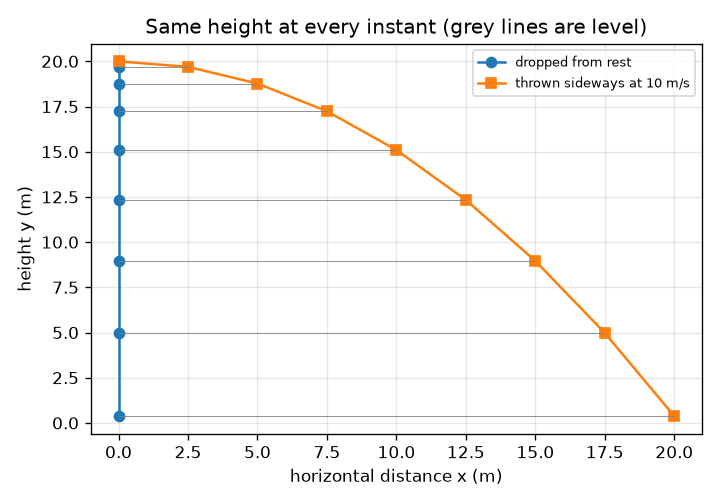
\includegraphics[width=0.85\linewidth]{figures/s01_independence.png}\\\small A dropped ball and a ball thrown sideways stay level with each other at every instant.\end{center}

\subsection*{E. Worked example}
A ball leaves the ground at 20 m/s at 30 degrees. Find its two velocity parts, the time of flight, the peak height and the range.
\begin{enumerate}[nosep]
\item vx = 20 cos 30 = 20 * 0.8660 = 17.32 m/s and vy = 20 sin 30 = 20 * 0.5 = 10.00 m/s.
\item Time of flight T = 2 vy / g = 2 * 10.00 / 9.81 = 2.04 s.
\item Peak height H = vy\textasciicircum{}2 / (2 g) = 100 / 19.62 = 5.10 m.
\item Range R = vx T = 17.32 * 2.039 = 35.3 m (keeping more digits gives 35.31 m).
\item Check: at t = T, y = 10.00 * 2.039 - 4.905 * 2.039\textasciicircum{}2 = 20.39 - 20.39 = 0, so the ball is back on the ground.
\end{enumerate}
\textbf{Answer.} vx = 17.32 m/s, vy = 10.00 m/s, T = 2.04 s, H = 5.10 m and R = 35.3 m.

\subsection*{F. Questions}
\begin{enumerate}[nosep]
\item \textbf{Conceptual.} One ball is dropped from rest and a second is thrown horizontally at 10 m/s from the same height at the same instant. Which hits the ground first? Explain.
\item \textbf{Numerical.} A ball is hit at 25 m/s at 36 degrees from the ground. Find vx, vy, the time of flight, the peak height and the range. Does the range look sensible?
\item \textbf{Graph and simulation interpretation.} In the app graph of x(t) and y(t) at 20 m/s and 30 degrees, what shape is each curve, and at what time does y return to zero? What does the slope of the x(t) line tell you?
\item \textbf{Design and optimisation challenge.} A keeper stands 35 m from a fielder who throws at 20 m/s. Using the app, find two different angles that both reach him. Compare the flights and say when you would choose each.
\end{enumerate}

\section{Session 2: The equations: range, best angle and a design problem}

\subsection*{A. Real-world problem}
A batter wants the ball to clear a boundary 70 m away. A fielder wants to hit the stumps from 50 m while the ball rises past a 10 m high gap. Guessing is slow. The equations of motion tell us exactly which speed and angle work, how many different ways there are, and which way needs the least effort.

\subsection*{B. Concept and theory}
Launch from height h0 at speed v and angle a. Then x = v cos(a) t and y = h0 + v sin(a) t - g t\textasciicircum{}2 / 2, with velocity vx = v cos(a) and vy = v sin(a) - g t. Removing t gives the path y = h0 + x tan(a) - g x\textasciicircum{}2 / (2 v\textasciicircum{}2 cos\textasciicircum{}2(a)), a parabola. Landing is y = 0, a quadratic in t whose positive root is T = (v sin(a) + sqrt(v\textasciicircum{}2 sin\textasciicircum{}2(a) + 2 g h0)) / g. The range is R = v cos(a) T. On level ground (h0 = 0) this becomes R = v\textasciicircum{}2 sin(2a) / g, using sin(2a) = 2 sin(a) cos(a). Since sin(2a) is at most 1, the best angle is 45 degrees and the longest range is v\textasciicircum{}2 / g. For a given range sin(2a) = g R / v\textasciicircum{}2 has two solutions, a and 90 - a. Launching from height h0 makes the best angle smaller: tan(a) = v / sqrt(v\textasciicircum{}2 + 2 g h0). To hit a target d metres away and h metres above the launch point, put x = d, y = h in the path equation with u = tan(a); a real u exists only if the speed is at least v\_min, where v\_min\textasciicircum{}2 = g (h + sqrt(d\textasciicircum{}2 + h\textasciicircum{}2)).

\begin{itemize}[nosep]
\item v: launch speed (m/s)
\item a: launch angle (degrees)
\item h0: launch height above the ground (m)
\item g: acceleration of gravity (9.81) (m/s\textasciicircum{}2)
\item R, T, H: range, time of flight, peak height (m, s, m)
\item d, h: target distance and height above the launch point (m)
\item v\_min: lowest speed that can reach the target (m/s)
\end{itemize}

\begin{equation*}
x=v\cos a\,t,\qquad y=h_0+v\sin a\,t-\tfrac12 g t^2
\end{equation*}

\begin{equation*}
y=h_0+x\tan a-\frac{g\,x^2}{2v^2\cos^2 a}
\end{equation*}

\begin{equation*}
T=\frac{v\sin a+\sqrt{v^2\sin^2 a+2gh_0}}{g},\qquad R=v\cos a\,T
\end{equation*}

\begin{equation*}
R=\frac{v^2\sin 2a}{g}\quad(h_0=0),\qquad \sin 2a=\frac{gR}{v^2}\ \Rightarrow\ a\ \text{and}\ 90^\circ-a
\end{equation*}

\begin{equation*}
\tan a_{\rm best}=\frac{v}{\sqrt{v^2+2gh_0}},\qquad v_{\min}^2=g\left(h+\sqrt{d^2+h^2}\right),\quad \tan a=\frac{h+\sqrt{d^2+h^2}}{d}
\end{equation*}

\begin{center}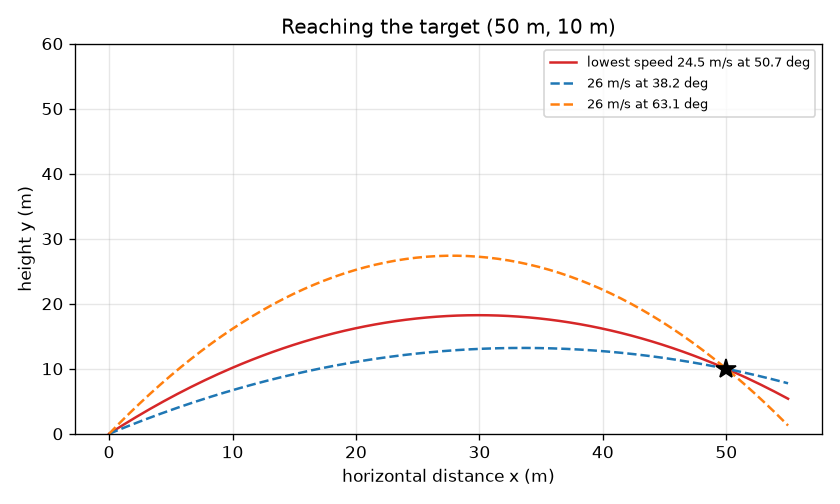
\includegraphics[width=0.85\linewidth]{figures/s02_hit_target.png}\\\small The lowest-speed path and the two 26 m/s paths that pass through the target (50 m, 10 m).\end{center}

\subsection*{E. Worked example}
A ball is launched at 25 m/s at 35 degrees from the ground. Find the time of flight, peak height and range. How much farther does it go if it is launched from a height of 1.5 m?
\begin{enumerate}[nosep]
\item vx = 25 cos 35 = 20.48 m/s and vy = 25 sin 35 = 14.34 m/s.
\item T = 2 vy / g = 2 * 14.34 / 9.81 = 2.92 s.
\item H = vy\textasciicircum{}2 / (2 g) = 205.6 / 19.62 = 10.48 m.
\item R = vx T = 20.48 * 2.923 = 59.87 m. Check with the formula: v\textasciicircum{}2 sin 70 / g = 625 * 0.9397 / 9.81 = 59.87 m.
\item From 1.5 m: T = (14.34 + sqrt(14.34\textasciicircum{}2 + 2 * 9.81 * 1.5)) / 9.81 = (14.34 + 15.33) / 9.81 = 3.02 s, so R = 20.48 * 3.025 = 61.94 m, which is 2.07 m farther.
\end{enumerate}
\textbf{Answer.} T = 2.92 s, H = 10.48 m, R = 59.87 m from the ground; from 1.5 m the range is 61.94 m, an extra 2.07 m.

\subsection*{F. Questions}
\begin{enumerate}[nosep]
\item \textbf{Conceptual.} Why is 45 degrees the best angle on level ground, and why do two different angles reach the same range?
\item \textbf{Numerical.} At 25 m/s, which launch angles give a range of 50 m on level ground? What is the maximum range at this speed?
\item \textbf{Graph and simulation interpretation.} In the range-versus-angle graph at 30 m/s, what do the grey and blue curves show, and where would you read two angles for R = 80 m?
\item \textbf{Design and optimisation challenge.} Design: you must hit a target 50 m away and 10 m above the launch point. What is the lowest possible speed, and at what angle? If you may use 26 m/s, which of the two available angles would you choose and why?
\end{enumerate}

\section{Session 3: Air drag: an RK4 simulation, validated}

\subsection*{A. Real-world problem}
In Sessions 1 and 2 the ball flew in a perfect parabola. A real cricket ball is slowed by the air: a hit that the formula says will travel 125 m may fall near 84 m. There is no neat formula any more, so we solve the motion step by step on the computer. But how do we know the answer is right? We test the solver on cases we can solve by hand: with drag switched off it must give Session 2's numbers exactly, and with drag on the energy books must balance. Only then do we use it to plan a shot.

\subsection*{B. Concept and theory}
Air pushes against the ball's velocity relative to the air, v\_rel, with a force that grows with its square: F = -k \textbar{}v\_rel\textbar{} v\_rel, where k = (1/2) rho Cd A, rho is the air density, Cd the drag coefficient and A = pi d\textasciicircum{}2 / 4 the cross-section. Dividing by the mass gives the acceleration a = -(k/m) \textbar{}v\_rel\textbar{} v\_rel + (0, -g). With a wind of speed w along +x, v\_rel = (vx - w, vy). We solve this by RK4: from the state (x, y, vx, vy) it takes one step of size dt by sampling the rate of change four times (start, two midpoints, end) and blending them with weights 1, 2, 2, 1 over 6; its error shrinks like dt\textasciicircum{}4 while explicit Euler (one sample) shrinks like dt. The landing moment is found by bisection inside the last step. Validation 1: with Cd = 0 the result must equal the exact formulas of Session 2. Validation 2: mechanical energy E = m g y + m v\textasciicircum{}2 / 2 changes only through drag, so E plus the work done against the ball by drag must stay constant; the solver integrates that work as an extra variable. Terminal speed is where drag balances weight: v\_t = sqrt(2 m g / (rho Cd A)).

\begin{itemize}[nosep]
\item m: mass of the ball (0.16, approximate) (kg)
\item d: diameter of the ball (0.07, approximate) (m)
\item Cd: drag coefficient (0.4, approximate, typical value) (no unit)
\item rho: air density (1.2 at sea level, approximate) (kg/m\textasciicircum{}3)
\item A: cross-section area, pi d\textasciicircum{}2 / 4 = 0.003848 (m\textasciicircum{}2)
\item k: drag constant, (1/2) rho Cd A (kg/m)
\item w: wind speed along the pitch (+ = tailwind) (m/s)
\item v\_t: terminal speed (m/s)
\item dt: time step of the solver (s)
\end{itemize}

\begin{equation*}
\mathbf F_{\rm drag}=-k\,|\mathbf v_{\rm rel}|\,\mathbf v_{\rm rel},\qquad k=\tfrac12\rho C_d A,\quad A=\frac{\pi d^2}{4}
\end{equation*}

\begin{equation*}
\ddot{\mathbf r}=-\frac{k}{m}\,|\mathbf v_{\rm rel}|\,\mathbf v_{\rm rel}+(0,-g),\qquad \mathbf v_{\rm rel}=(v_x-w,\ v_y)
\end{equation*}

\begin{equation*}
\mathbf s_{n+1}=\mathbf s_n+\frac{\Delta t}{6}\left(\mathbf k_1+2\mathbf k_2+2\mathbf k_3+\mathbf k_4\right)\quad\text{(RK4)}
\end{equation*}

\begin{equation*}
E(t)+W_{\rm drag}(t)=E(0),\qquad E=mgy+\tfrac12 mv^2
\end{equation*}

\begin{equation*}
v_t=\sqrt{\frac{2mg}{\rho C_d A}}
\end{equation*}

\begin{center}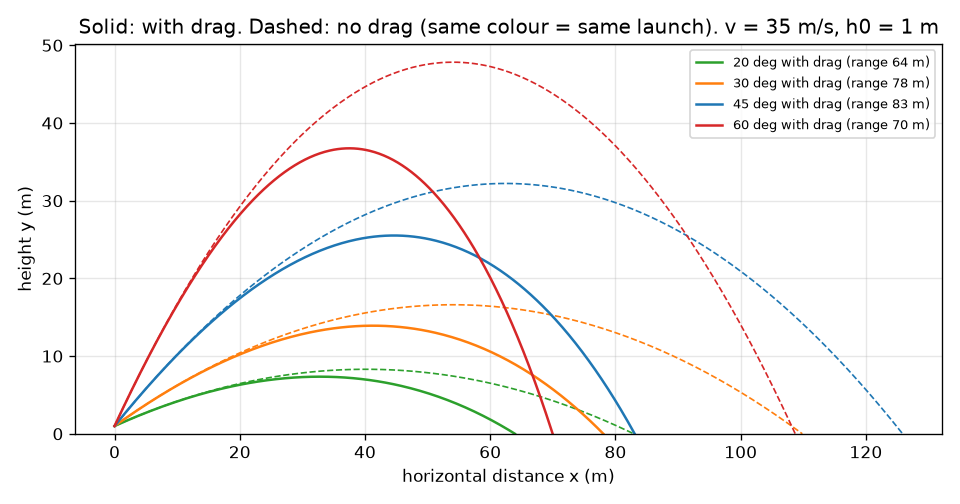
\includegraphics[width=0.85\linewidth]{figures/s03_drag_vs_vacuum.png}\\\small Four launch angles at 35 m/s with drag (solid) and without (dashed).\end{center}

\subsection*{E. Worked example}
A cricket ball (m = 0.16 kg, d = 0.07 m, Cd = 0.4, approximate) is hit from 1 m at 35 m/s and 40 degrees. Find k, the terminal speed, the drag deceleration at launch, and then the range from the RK4 solver.
\begin{enumerate}[nosep]
\item A = pi * 0.07\textasciicircum{}2 / 4 = 0.003848 m\textasciicircum{}2.
\item k = 0.5 * 1.2 * 0.4 * 0.003848 = 9.24e-4 kg/m, so k/m = 9.24e-4 / 0.16 = 0.00577 per metre.
\item Terminal speed v\_t = sqrt(2 * 0.16 * 9.81 / (1.2 * 0.4 * 0.003848)) = sqrt(1699.5) = 41.2 m/s.
\item Drag deceleration at launch = (k/m) v\textasciicircum{}2 = 0.00577 * 35\textasciicircum{}2 = 7.07 m/s\textasciicircum{}2, which is 0.72 g: air matters a lot at this speed.
\item RK4 (dt = 0.01 s) gives a range of 83.5 m, a flight of 4.14 s and a peak of 21.6 m. With drag off the same hit gives 124.2 m, 4.63 s and 26.8 m (the exact formulas agree to better than a micrometre), so drag costs 40.7 m, about a third of the range.
\item Energy check: E + W\_drag differs from E(0) by a relative 2e-12 along the whole flight, as it should for a correct solver.
\end{enumerate}
\textbf{Answer.} k = 9.24e-4 kg/m, v\_t = 41.2 m/s, launch drag deceleration 7.07 m/s\textasciicircum{}2, and with drag the range is 83.5 m (124.2 m without drag).

\subsection*{F. Questions}
\begin{enumerate}[nosep]
\item \textbf{Conceptual.} Why does air drag lower the best launch angle below 45 degrees? Think about what a high, long flight costs.
\item \textbf{Numerical.} For a slightly rougher ball with Cd = 0.5 (same mass and diameter), find k, the terminal speed, and the drag deceleration at 30 m/s as a multiple of g.
\item \textbf{Graph and simulation interpretation.} In the range-versus-angle graph at 35 m/s from 1 m, the dashed (no drag) curve peaks at 44.8 degrees and 125.9 m, the solid curve at 41.5 degrees and 83.6 m. What percentage of the range does drag remove and what happens to the shape of the peak?
\item \textbf{Design and optimisation challenge.} Design: the rope is 70 m from the batter and the ball is struck from 1.0 m. Find the lowest speed that makes a six in still air, and say what speed and angle you would plan for a 5 m/s headwind. Comment on the margin.
\end{enumerate}

\section{Real-world mini-project}
\textbf{Clear the boundary rope for a six.} Illustrative numbers: the boundary rope is 70 m from the batter and the ball is struck from a height of 1.0 m. The ball counts as a six if it reaches the rope before it touches the ground. Use the cricket ball of Session 3 (mass 0.16 kg, diameter 0.07 m, Cd 0.4, approximate). Find the lowest launch speed (rounded up to 0.1 m/s) that can make a six, and the angle it needs. Compare it with the no-drag answer of Session 2. Then repeat for a 5 m/s headwind and a 5 m/s tailwind, and list the whole-degree angles that clear the rope at 32 m/s.

\section{The path ahead}
\begin{enumerate}[nosep]
\item \textbf{Session 4: Bounce and roll.} A flight that continues after the first landing with a bounce model (illustrative: vertical speed halved, horizontal speed times 0.8).
\item \textbf{Session 5: Crosswind in 3D.} A 3D version of the solver with a sideways wind.
\item \textbf{Session 6: Fit the drag coefficient from a video.} A least-squares fit of Cd to simulated camera points (positions every 0.1 s with 0.2 m of noise).
\item \textbf{Session 7: The optimal-angle map, fast.} A map of the best angle over 26 launch speeds (10 to 60 m/s) and 21 drag coefficients (0 to 0.8).
\item \textbf{Session 8: A shot planner with uncertainty.} A function that reports the lowest and highest range for Cd between 0.35 and 0.45 and wind between -3 and +3 m/s.
\end{enumerate}

\section{Answers and hints}

\subsection*{Session 1}
\begin{enumerate}[nosep]
\item \textbf{Conceptual.} Hint: Look at the formula for y: does it contain the sideways speed? Solution: They land at the same moment. The height formula y = y0 - g t\textasciicircum{}2 / 2 has no sideways speed in it: gravity acts only vertically and does not care how fast the ball moves sideways. The thrown ball simply covers more ground while it falls.
\item \textbf{Numerical.} Hint: sin 36 = 0.588 and cos 36 = 0.809. Then T = 2 vy / g. Solution: vx = 25 * 0.809 = 20.23 m/s and vy = 25 * 0.588 = 14.69 m/s. T = 2 * 14.69 / 9.81 = 3.00 s. H = 14.69\textasciicircum{}2 / 19.62 = 11.0 m. R = 20.23 * 3.00 = 60.6 m. Sanity check: a hit of 25 m/s (about 90 km/h) going 60 m is a plausible, if a little long, no-air figure; with air it will be shorter (Session 3). Units: m/s * s = m.
\item \textbf{Graph and simulation interpretation.} Hint: One formula has t, the other has t\textasciicircum{}2. Solution: x(t) = vx t is a straight line; its slope is the constant sideways speed 17.32 m/s. y(t) = vy t - g t\textasciicircum{}2 / 2 is a parabola opening downwards; it returns to zero at T = 2.04 s, half way (1.02 s) it peaks at 5.10 m. The straight line against the curve is the independence of the two motions.
\item \textbf{Design and optimisation challenge.} Hint: Try 30 degrees, then look for a second angle that gives the same range. Solution: 30 and 60 degrees both give a range of 35.3 m at 20 m/s. At 30 degrees the flight takes 2.04 s and peaks at 5.1 m: quick and low, best when a runner is going (but the ball arrives fast and flat). At 60 degrees it takes 3.53 s and peaks at 15.3 m: slow, easy to catch as it drops steeply, but it gives a runner more time. Assumption: no air, equal heights.
\end{enumerate}

\subsection*{Session 2}
\begin{enumerate}[nosep]
\item \textbf{Conceptual.} Hint: R = v\textasciicircum{}2 sin(2a) / g. What are the largest value of sin(2a) and the symmetry of the sine curve? Solution: R is proportional to sin(2a), which is largest (1) when 2a = 90 degrees, so a = 45. The sine curve is symmetric about 90 degrees, so 2a and 180 - 2a give the same sin value, i.e. a and 90 - a give the same range. A low flat shot and a high lofted shot land together. At exactly 45 the two merge into one.
\item \textbf{Numerical.} Hint: sin(2a) = g R / v\textasciicircum{}2 = 9.81 * 50 / 625. Solution: sin(2a) = 490.5 / 625 = 0.7848, so 2a = 51.7 degrees (or 128.3), giving a = 25.85 and 64.15 degrees. Check: they add up to 90. Maximum range is v\textasciicircum{}2 / g = 625 / 9.81 = 63.7 m at 45 degrees; 50 m is below it, so two angles exist.
\item \textbf{Graph and simulation interpretation.} Hint: Draw a horizontal line at 80 m and see where it cuts the curve. Solution: The grey curve is a launch from the ground (peak 91.7 m at 45 degrees), the blue curve is a launch from the chosen height (higher everywhere, peak slightly left of 45). A horizontal line at 80 m cuts the ground curve at 30.3 and 59.7 degrees: two angles that add up to 90. Units: range in metres, angle in degrees.
\item \textbf{Design and optimisation challenge.} Hint: Use v\_min\textasciicircum{}2 = g (h + sqrt(d\textasciicircum{}2 + h\textasciicircum{}2)). At 26 m/s solve the quadratic in tan(a) (lesson function \texttt{angles\_to\_hit}). Solution: v\_min\textasciicircum{}2 = 9.81 * (10 + sqrt(2500 + 100)) = 9.81 * 60.99 = 598.3, so v\_min = 24.46 m/s at tan(a) = 60.99 / 50, a = 50.65 degrees; below this speed no angle works. At 26 m/s there are two: 38.24 degrees (flight 2.45 s, peak 13.2 m) and 63.07 degrees (flight 4.25 s, peak 27.4 m). The flat shot is faster to arrive and gives the fielder less time to react but it needs a clear low path; the high shot is slower, but arrives steeply and needs more height clearance. At exactly v\_min there is one angle and no margin for error, so the extra speed is a safety margin. Assumption: no air.
\end{enumerate}

\subsection*{Session 3}
\begin{enumerate}[nosep]
\item \textbf{Conceptual.} Hint: Drag removes speed all the time the ball is in the air. Which shot spends longer in the air? Solution: Drag keeps slowing the ball for as long as it is flying, and it acts most when the ball is fast. A lofted shot stays in the air longer, so it loses more speed (and more sideways speed in particular) than in a vacuum. Lowering the angle trades a little height for a shorter flight and less time under drag, so the longest range moves to a smaller angle. The effect grows with speed: 44.3 degrees at 15 m/s, 41.8 at 35 m/s and 38.6 at 60 m/s (from level ground).
\item \textbf{Numerical.} Hint: k = 0.5 rho Cd A with A = 0.003848 m\textasciicircum{}2; deceleration = (k/m) v\textasciicircum{}2. Solution: k = 0.5 * 1.2 * 0.5 * 0.003848 = 1.155e-3 kg/m. v\_t = sqrt(2 * 0.16 * 9.81 / (1.2 * 0.5 * 0.003848)) = sqrt(1359.6) = 36.9 m/s. Deceleration = (1.155e-3 / 0.16) * 900 = 6.49 m/s\textasciicircum{}2 = 0.66 g. Sanity check: higher Cd gives a lower terminal speed (36.9 against 41.2 m/s for Cd = 0.4) and a larger drag, as expected.
\item \textbf{Graph and simulation interpretation.} Hint: Percentage lost = (125.9 - 83.6) / 125.9. Solution: Loss = 42.3 / 125.9 = 33.6 percent. The solid peak is lower and moves left (about 3.3 degrees); drag hurts high shots more than flat ones. Units: metres and degrees.
\item \textbf{Design and optimisation challenge.} Hint: Use \texttt{min\_speed\_for\_range(70, 1.0)} and \texttt{angle\_window} from the lesson; repeat with wind = -5. Solution: In still air the lowest speed is 30.9 m/s (rounded up) at about 42.0 degrees; ignoring drag you would wrongly plan 26.0 m/s, which falls about 16 m short (54 m). With a 5 m/s headwind it is 33.5 m/s (best angle about 39.4 degrees); a 5 m/s tailwind needs 29.1 m/s. At the exact lowest speed there is no margin: at 31 m/s the clearing angles are only 39 to 45 degrees, at 32 m/s they widen to 32 to 52 degrees. So plan for a few m/s above the minimum and a launch angle near 40 degrees,. Assumptions: illustrative numbers, a point ball, steady wind, approximate Cd.
\end{enumerate}

\section{How to join}
Read \texttt{CONTRIBUTING.md} in the repository, then pick an issue labelled \texttt{good first issue}. Repository: \url{https://github.com/KrunalPanchal1995/pan-iit-oss/tree/main/openprojectile}

\end{document}
